\documentclass[a4paper, 12pt]{extarticle}
\usepackage[dvipsnames]{xcolor}
\usepackage[top=70pt,bottom=70pt,left=48pt,right=46pt]{geometry}
\definecolor{header}{RGB}{252, 171, 16}
\definecolor{defenition}{RGB}{248, 51, 60}
\definecolor{main_title}{RGB}{43, 158, 179}
\definecolor{sub_header}{RGB}{68, 175, 105}
\usepackage[english, russian]{babel}
\usepackage[utf8]{inputenc}
\usepackage{amsmath}
\usepackage[most]{tcolorbox}
\usepackage{listings}
\usepackage{graphicx}
\usepackage{amsmath}
\usepackage{lettrine}
\title{\textcolor{main_title}{Пространственные характеристики излучения полупроводникового инжекционного лазера}}
\author{Шмаков Владимир Евгеньевич - ФФКЭ гр. Б04-103}


\newtcolorbox{fequation}[1][]{ams equation,size=small,#1}








\begin{document}
\maketitle



\section*{\textcolor{header}{Цель работы}}

\begin{itemize}
    \item Исследование диаграмм направленности полупроводникового лазера.
    \item Нахождение геометрических размеров активного слоя лазера.
    \item Исследование диаграмм направленности светодиода.
\end{itemize}

\section*{\textcolor{header}{Теоретические сведения}}

\begin{figure}[htbp]
    \centering
    \includegraphics[width = 0.9\textwidth]{pics/setup_1.png}
    \caption{Пространственные характеристики излучения полупроводникового инжекционного лазера}
    \label{fig:1}
\end{figure}

На рисунке \ref{fig:1} представлена схема полупроводникового инжекционного лазера. Полупроводниковый инжекционный лазер состоит из \textit{p-n} перехода, активной области и резонатора. При подаче прямого напряжения электроны из \textit{n}-области и дырки из \textit{p}-области инжектируются в активную область, где происходит их рекомбинация с испусканием фотонов. В качестве резонатора обычно используются сколотые грани кристалла.



\begin{figure}[htbp]
    \centering
    \includegraphics[width = 0.7\textwidth]{pics/difraction.jpg}
    \caption{Излучение, выходящие из активного слоя под углом $\phi$.}
    \label{fig:difr}
\end{figure}
Диаграмма направленности излучения полупроводникового лазера возникает из-за дифракции света, покидающего активную область(рисунок \ref{fig:difr}).

В направлении, перпендикулярном p-n переходу (высота активной области мала), излучение сильно расходится. В направлении, параллельном p-n переходу (ширина активной области больше), расходимость излучения меньше. В результате диаграмма направленности лазера имеет эллиптическую форму: пучок узкий в одной плоскости и широкий в другой(смотрите рисунок \ref{fig:1}).

Найдём сумму волн, исходящих из активного слоя в направлении $\phi$(формула \ref{eq:integral}).
\begin{equation}
    \label{eq:integral}
    S = \int_{-d / 2}^{d / 2} E(x) e^{i k x \sin(\phi)} dx    
\end{equation}
Распределение напряжённости поля в волноводе описывается функциями вида \( E(x) \sim \sin(qx) \) или \( E(x) \sim \cos(qx) \), в зависимости от типа моды электромагнитного поля. Подставим $E(x)$ в выражение \ref{eq:integral} и проинтегрируем(формулы \ref{eq:main_odd} и \ref{eq:main_even}).
\begin{equation}    
    \label{eq:main_odd}
    S(\varphi) \sim \frac{\cos \left( \frac{\pi d}{\lambda} \sin \varphi \right)}
    {\left( \frac{\lambda (m+1)}{2d} \right)^2 - \sin^2 \varphi} - \text{четные моды\\}
\end{equation}

\begin{equation}
    \label{eq:main_even}
    S(\varphi) \sim \frac{\sin \left( \frac{\pi d}{\lambda} \sin \varphi \right)}
    {\left( \frac{\lambda (m+1)}{2d} \right)^2 - \sin^2 \varphi} - \text{нечетные моды}
\end{equation}


Возведя выражения \ref{eq:main_even} и \ref{eq:main_odd} в квадрат получаем энергетическую диаграмму направленности излучения диода. Анализируя выражение \ref{eq:main_odd} можно получить связь между шириной активного слоя и угловой шириной диаграммы направленности на уровне 0.6 при $m = 0$:

\begin{fequation}
d = \frac{\lambda}{2 \sin(\phi_{0.6})}
\end{fequation}


\section*{\textcolor{header}{Методика}}
\subsection*{\textcolor{sub_header}{Оборудование}}
\begin{itemize}
    \item Полупроводниковый инжекционный лазер
    \item Фотоприёмник
    \item Генератор импульсов
    \item Светодиод
    \item Узкополосный усилитель
    \item Блок питания
    \item Вращательный привод
    \item Транспортир
\end{itemize}

\subsection*{\textcolor{sub_header}{Экспериментальная установка}}

\begin{figure}[htbp]
    \centering
    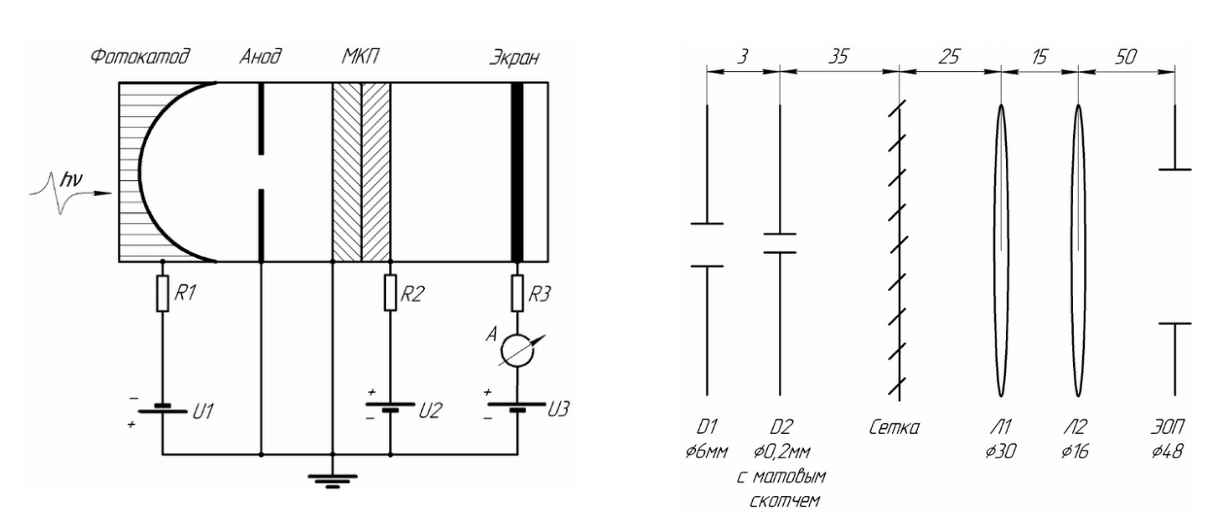
\includegraphics[width = 0.9\textwidth]{pics/experimental_setup.png}
    \caption{Блок - схема экспериментальной установки}
    \label{fig:exp_setup}
\end{figure}


Блок - схема экспериментальной установки изображена на рисунке \ref{fig:exp_setup}. Излучение исследуемого лазера(1) фиксируется при помощи фотоприёмника(5). Лазер установлен на вращающемся приводе. Угол поворота лазера фиксируется при помощи транспортира. 

Для <<отсечения>> внешней засветки используется следующая методика:
    \begin{itemize}
        \item Накачка лазера осуществляется меандром некоторой частоты $w$. Для получения меандра используется генератор импульсов(3).
        \item Сигнал фотоприёмника проходит через узкополосный фильтр(6), центральная частота которого совпадает с частотой меандра $w$. 
    \end{itemize}

\section*{\textcolor{header}{Обработка экспериментальных данных}}
\subsection*{\textcolor{sub_header}{Диаграмма направленности излучения лазера при токе накачки $65$мкА}}


При токе накачки $J_p = 65 \text{мкА}$ сняли диаграммы направленности излучения лазера в двух плоскостях - параллельной активному слою ($ZY$) и перпендикулярной активному слою($XZ$). Экспериментальные данные могут быть найдены в приложении(таблицы \ref{tab:ZY_65} и \ref{tab:XZ_65}). Полученные в ходе эксперимента кривые изображены на рисунках \ref{fig:ZY_65} и \ref{fig:XZ_65}.

\begin{figure}[htbp]
    \centering
    \includegraphics[width = 0.9\textwidth]{pics/lazer_horizonta_65.png}
    \caption{Диаграмма направленности излучения лазера в плоскости ZY. Ток накачки $J_p = 65\text{мкА}$.}
    \label{fig:ZY_65}
\end{figure}

Для нахождения ширины кривой, интерполируем её сплайнами степени 1. Пусть $f(\gamma)$ построенный интерполянт. Задача нахождения ширины экспериментальной кривой свелась к поиску корней уравнения $f(\gamma) = 0.6 \max_{\gamma} f(\gamma)$. Корни уравнения $\gamma_l$ и $\gamma_r$ изображены на легендах графиков(рисунки \ref{fig:ZY_65}, \ref{fig:XZ_65}).



\begin{figure}[htbp]
    \centering
    \includegraphics[width = 0.9\textwidth]{pics/vertical_65_muA.png}
    \caption{Диаграмма направленности излучения лазера в плоскости $XZ$. Ток накачки $J_p = 65\text{мкА}$.}
    \label{fig:XZ_65}
\end{figure}

Ширина кривой позволяет оценить размеры активного слоя лазера(формула 4). Ширина активного слоя(размер вдоль оси $Y$) оказалась равной:
$$
d = \frac{\lambda}{2 \sin(\gamma_r - \gamma_l)} = \frac{635 \text{нм}}{2 \sin(18.62^{\circ})} \sim 1 \text{мкм}
$$

Высота активного слоя(размер вдоль оси $X$) оказалась равной:
$$
h = \frac{\lambda}{2 \sin(\gamma_r - \gamma_l)} = \frac{635 \text{нм}}{2 \sin(5.7^{\circ})} \sim 3.2 \text{мкм}
$$

Длина волны лазера $\lambda$ была принята равной $635\text{нм}$, поскольку это характерная длина волны излучения материала активной среды $InGaP$, часто используемого при изготовлении светодиодов и лазерных указок.


\subsection*{\textcolor{sub_header}{Диаграмма направленности излучения лазера при токе накачки $51$мкА}}

При токе накачки $J_p$ была получена диаграмма направленности излучения лазера в плоскости $ZY$. Экспериментальные данные могут быть найдены в приложении(таблица \ref{tab:ZY_51}). Экспериментально полученная кривая изображена на рисунке  \ref{fig:ZY_51}.

\begin{figure}[htbp]
    \centering
    \includegraphics[width = 0.9\textwidth]{pics/lazer_horizontal_51.png}
    \caption{Диаграмма направленности излучения лазера в плоскости $ZY$. Ток накачки $J_p = 51\text{мкА}$.}
    \label{fig:ZY_51}
\end{figure}

Пользуясь описанной в предыдущем пункте методикой, оценим ширину активного слоя лазера.
$$
d = \frac{\lambda}{2 \sin(\gamma_r - \gamma_l)} = \frac{635 \text{нм}}{2 \sin(19.5^{\circ})} \sim 0.95 \text{мкм}
$$

\subsection*{\textcolor{sub_header}{Диаграмма направленности излучения светодиода}}

Была получена диаграмма направленности излучения светодиода(рисунках \ref{fig:diode}). Экспериментальные данные могут быть найдены в приложении(таблица \ref{tab:diode}).

\begin{figure}[htbp]
    \centering
    \includegraphics[width = 0.8\textwidth]{pics/diode.png}
    \caption{Диаграмма направленности излучения светодиода}
    \label{fig:diode}
\end{figure}

Экспериментальная методика не обеспечивает точного определения геометрических размеров диода. Помимо $p-n$ перехода, светодиод включает рассеивающую <<шляпку>> и отражатель, которые изменяют пространственное распределение излучения и искажают его диаграмму направленности.


На рисунке \ref{fig:diode} показано, что ширина угловой характеристики излучения составляет примерно \(7^\circ\). Это позволяет оценить ширину излучающей области $p$-$n$ перехода, которая составляет порядка нескольких микрон.


\subsection*{\textcolor{sub_header}{Модельная диаграмма направленности}}

\begin{figure}[htbp]
    \centering
    \includegraphics[width = 0.9\textwidth]{pics/model.png}
    \caption{Приближение экспериментальных данных модельной кривой.}
    \label{fig:model}
\end{figure}

Теоретически, угловое распределение интенсивности есть $S(\phi)^{2}$. Где $S$ задано формулами \ref{eq:main_odd} и \ref{eq:main_even}. Приблизим диаграмму направленности, представленной на рисунке \ref{fig:XZ_65} модельной кривой. Для этого:
\begin{itemize}
    \item Нормируем полученные в ходе эксперимента значения напряжения $V_i$: $J_i = V_i / (\max_i V_i)$. $i$ - номер измерения.
    \item Определим функцию потерь $L$, как $L = \sum_i (S(\gamma_i, d) / (\max_{i} S(\gamma_i, d)) - J_i)^{2}$ 
    \item Методом Нелдера - Мида определим оптимальный параметр $d$ и оптимальный сдвиг кривой $s$, при которых функция $L$ достигает минимума.
\end{itemize}


Результаты оптимизации изображены на рисунке \ref{fig:model}. Толщина активного слоя, минимизирующая функцию $L$, оказалась равной 3.2 мкн. Таким образом, толщина полученная в ходе оптимизации параметров модельной функции совпала с толщиной, рассчитанной по формуле 4.

\section*{\textcolor{header}{Вывод}}

\begin{itemize}
    \item Удалось оценить геометрические размеры активной области инжекционного полупроводникового лазера.
    \item Удалось найти порядок размера активной области полупроводникового светодиода.
    \item Диаграмма направленности излучения в плоскости $XZ$(перпендикулярной активному слою) с высокой точностью приближается модельной кривой.
    \item Диаграммы в плоскости $ZY$(параллельной активному слою) не могут быть приближены модельной кривой. Это связано с тем, что ширина активного слоя близка к длине волны, однако используемая математическая модель не учитывает дифракцию выходного пучка.
\end{itemize}

\newpage
\section*{\textcolor{header}{Приложение}}


\begin{table}[htbp]
    
\begin{center}

    \begin{tabular}{|l|l|}
        \hline
    Угол[$^{\circ}$]&Напряжение[В]\\
    \hline
    0&0.55\\
    1&0.58\\
    2&0.58\\
    3&0.59\\
    4&0.58\\
    5&0.58\\
    6&0.58\\
    7&0.57\\
    8&0.57\\
    9&0.56\\
    10&0.55\\
    11&0.53\\
    12&0.47\\
    13&0.03\\
    14&0\\
    -1&0.56\\
    -2&0.54\\
    -3&0.53\\
    -4&0.5\\
    -5&0.48\\
    -6&0.46\\
    -7&0.14\\
    -8&0\\
    -9&0\\
    \hline

    \end{tabular}
\end{center}
\caption{Излучение лазера в плоскости $ZY$. Ток накачки $J_p = 65\text{мкА}$.}
\label{tab:ZY_65}
\end{table}


\begin{table}
\begin{center}
    

\begin{tabular}{|l|l|}
    \hline
    Угол[$^{\circ}$]&Напряжение[В]\\
    \hline
0&0.56\\
1&0.7\\
2&0.72\\
3&0.68\\
4&0.59\\
5&0.44\\
6&0.26\\
7&0.14\\
8&0.1\\
9&0.02\\
10&0\\
-1&0.36\\
-2&0.25\\
-3&0.14\\
-4&0.07\\
-5&0\\
\hline
\end{tabular}

\end{center}
\caption{Излучение лазера в плоскости $XZ$. Ток накачки $J_p = 65\text{мкА}$.}
\label{tab:XZ_65}
\end{table}




\begin{table}
    \begin{center}
        

\begin{tabular}{|l|l|}
    \hline
    Угол[$^{\circ}$]&Напряжение[мВ]\\
    \hline
    0&5\\
    1&5.1\\
    2&5.2\\
    3&5.2\\
    4&5.2\\
    5&5.2\\
    6&5.2\\
    7&5.2\\
    8&5.1\\
    9&5\\
    10&4.9\\
    11&4.6\\
    13&2.4\\
    14&1.2\\
    15&1.2\\
    16&1.2\\
    -1&5\\
    -2&4.8\\
    -3&4.7\\
    -4&4.6\\
    -5&4.4\\
    -6&4.2\\
    -7&3.8\\
    -7.5&1.6\\
    -8&1\\
    -9&1\\
    -10&1\\
    \hline
\end{tabular}


    
    \end{center}
    \caption{Излучение лазера в плоскости $ZY$. Ток накачки $J_p = 51\text{мкА}$.}
    \label{tab:ZY_51}
    \end{table}
    

    
\begin{table}
    \begin{center}
            

        \begin{tabular}{|l|l|}
            \hline
            Угол[$^{\circ}$]&Напряжение[мВ]\\
            \hline
            0&82\\
            1&80\\
            2&71\\
            3&54\\
            4&38\\
            5&23\\
            6&16\\
            7&14\\
            8&13\\
            9&10\\
            10&10\\
            11&10\\
            -1&78\\
            -2&74\\
            -3&64\\
            -4&46\\
            -5&30\\
            -6&21\\
            -7&16\\
            -8&13\\
            -9&10\\
            -10&8\\
            -11&6\\
            -12&4\\
            -13&4\\
            -14&4\\
            \hline
        \end{tabular}

    \end{center}
    \caption{Диаграмма направленности излучения светодиода, сила тока $J = 70\text{мкА}$.}
    \label{tab:diode}
\end{table}
    
    
    



\end{document}
